\chapter{Artifact design and features} 

\label{Chapter5} 

\section{Design considerations and choices}

In this chapter, the critical thought processes and decisions that shape the application architecture are documented. By exploring this chapter, readers will gain insights into the rationale behind the artifact structure and the reasons for selecting particular solutions over others.

\subsection{Software category}

There are multiple options to implement an application to read and compile information from a digital SCRUM platform.
The most common and recommended ones include writing an extension for a specific platform and creating custom software that uses REST endpoints if the platform exposes any.

\subsubsection{Extension for a SCRUM platform}
The first design cycle will produce an artifact that will be used to extract data from the SCRUM platform Azure DevOps. Therefore an option would be to develop an extension for this platform.
Microsoft provides documentation on how to develop extensions for your organizational DevOps platform \footnote{\cite{AzureExtensions}}.
Simple authentication for users, storage provided by Azure and the accessibility of use speak in favor of this method.
The only downside, why it should be decided against, is that an extension for DevOps limits the functionality of the application to the Microsoft platform. If other things would also want to be integrated in the future, the application could not be extended in such a way that it also works with external applications. In addition, only developers could evaluate sprints and view the results because a Visual Studio license is required to access the platform.

\subsubsection{Independent application}
An independent application can access work items and sprint info via a REST API provided by the most used SCRUM platforms like Atlassian Jira and Azure DevOps \parencite{TopTenScrum}. If needed in the future, more platforms can be integrated into this application and it could be hosted anywhere. Another advantage is the free choice of the implementation language, which makes it much easier for a company to expand the application at a later date. A disadvantage is that the application has to be written from scratch. This means that communication with Azure services, user authentication, and data storage must both be designed and implemented. Nevertheless, it is a favorable choice.

\subsection{Application architecture}

In the early stages of designing the artifact, an important decision is the adoption of a distributed application architecture by separating the front-end, back-end, and database into containerized parts. This choice is influenced by several factors backed by research. One paper explores the performance of traditional VM deployments and contrasts them with the use of Linux containers. The authors used KVM as a representative hypervisor and Docker as a container manager. The results show that containers result in equal or better performance than VMs in almost all cases \parencite{felter2015updated}. Another study compares the performance of Docker containers and VMs using different cloud vendors. Docker containers are found to be faster than KVMs and Xen VMs in terms of response time, download time, CPU processing time, and memory usage. The performance of Docker containers improves when scaled using the Kubernetes framework \parencite{chengeta2021comparing} which will also be the hosting choice for first evaluating the artifact. Relevant to this thesis and the decision made are the following points:

\begin{itemize}
    \item \textbf{Personal experience}: Familiarity with the technology stack is invaluable. Having prior experience with distributed systems and containers ensured a smoother development process.
    \item \textbf{Modern technology}: Distributed applications, especially when combined with containers, represent the cutting edge in software architecture. 
    \item \textbf{Scalable components}: One of the primary advantages of a distributed application is its scalability. Although it's not important for this thesis it's nice to have the option to scale as demand gets higher.
    \item \textbf{High availability}: Distributed architectures tend to offer better fault tolerance. Containerization further enhances this by allowing rapid redeployment of single components, ensuring minimal downtime.
    \item \textbf{Independence}: Containerization makes sure every component runs in a consistent environment. This encapsulation allows for flexibility in development as each component can be developed and tested independently.
    \item \textbf{Resource efficiency}: Containers are lightweight compared to traditional virtual machines. This means they start quickly and use fewer system resources. Multiple containers can be deployed onto a single machine which means that resources can be used more efficiently.
    \item \textbf{Consistent environments}: Containerization ensures that the application runs the same, regardless of where the container is deployed. This consistency can reduce the "it works on my machine" type of issues. 
\end{itemize}

\subsection{Programming languages and frameworks}

Selecting a programming language for a project is often influenced by the developer's previous experience. In many cases, developers lean towards languages they are already familiar with. This eliminates the need to learn a new language. This preference is not just a matter of comfort but also efficiency. Using a programming language known by the developer reduces errors, saves time, and enhances the quality of the final artifact. Since the application is split into three parts two programming languages and frameworks have to be selected in addition to a database system.


\subsubsection{Back-end}

The heart of the application is its API which is used to create and evaluate KPIs, issue and review Reports, and define dashboards for report presentation to a SCRUM team. ASP.NET is selected for this part of the application, which is a web application framework developed by Microsoft. ASP.NET is built on the Common Language Runtime (CLR), which means developers can write ASP.NET code using any supported .NET language like C\#, VB.NET, and F\#. The choice for this project is to use ASP.NET with C\# \footnote{ASP.NET documentation: \cite{ASPNETDocumentation}}.

\subsubsection{Database}

A relational database is used to store reports, KPIs, and other models that are needed for the application. The choice of provider is PostgreSQL because it's open source and easy to use with ASP.NET. the database schema is implemented code-first using an Object-Relational Mapping (ORM) framework for ASP.NET called Entity Framework. This framework automatically takes care of any migrations that may need to be issued to the schema and allows incremental creation of the model code first.

\subsubsection{Front-end}

To present sprint metrics and data, configure how data is retrieved, and manage user access a user interface is essential.
The front end of the application is coded in Typescript with the extended capabilities of the library React by Facebook \footnote{React by Facebook: \cite{ReactDev}}. The user interface provides a method for the user to interact with the back-end API using controls rather than web requests which makes the application more accessible.  

\subsubsection{Composition}

The final artifact consists of three docker images: one for the front-end of the application, one for the back-end, and one for the database\footnote{Docker: \cite{DockerGetStarted}}.
Locally, this can be run via a provided 'docker-compose' file but in production, these images need to be hosted separately and configured in such a way that they know each other's location.

\subsection{Capabilities}

A rather weak form of use cases and requirements is added to the design of the artifact in the beginning to give an idea about the application's capabilities. This determines the starting point for model design and use cases. This definition is loosely written on paper at first and then reworked into use cases and requirements as soon as the model is designed. The artifact should be able to store templates for report creation. That means it should allow users to create templates or models to base their reports on. These templates should include information on how to get data and compute KPIs. The application should also provide the possibility to create graphical dashboards to present reports. Reports should also be comparable to other reports. Users should be able to manage who has access to their templates and what actions they can take in the context of their templates. The user creation and authentication are not handled by the application itself. Users are allowed to authenticate using OAUTH\footnote{https://oauth.net/2/}.

\section{Model}

This section dives into the system's structure and its intended operations. First, the model is presented, detailing the primary components. Following that, various use cases illustrate the system in action, providing a comprehensive understanding of its functionality and interactions.

\subsection{Data model}

A central part of this application will be the data model behind it. Before actually implementing this model it is sketched out on paper. This step ensures that there is a clear picture of how the data elements relate and interact with each other. By mapping things out early, one can pinpoint potential issues and make necessary adjustments. Essentially, it's about laying a strong foundation from the get-go to ensure the app's long-term efficiency and adaptability. When the sketch is finished the model will be implemented code-first using an ORM tool to map the coded model into a relational database. This section will provide information on how the model is planned and structured. Most models will have a property called \code{Id} in which they store a GUID value as the primary key for the relational database mapping. The diagrams presented in this section were designed with the UML standard \footnote{\cite{uml_standard}} in mind. However, it is worth noting that while every effort is made to comply with the UML conventions there might be subtle differences in the representation. These discrepancies arise from the limitations of the LaTeX environment as well as translating complex software designs into visual format. Readers familiar with UML should interpret the diagrams with a degree of flexibility as the goal is just to convey the structure of the data model.
 
\subsubsection{Analysis models}

The idea of this application is to have a way to design a schema or model that can be followed to evaluate performance indicators about a SCRUM sprint. The \code{AnalysisModel} data class is designed to do just that. It holds information about how to get and evaluate data. It also includes configuration on how to visualize data to present it to team members. A graphical representation shows the most important parts of the model in \ref{fig:kpis-and-models} after a brief description in the next paragraphs.

KPIs are an essential part of this thesis and have to be included in the data model. The classes \code{KPI} and \code{Expression} are designed to store details about KPIs and how to evaluate them. Also included in the \code{KPI} class is the configuration of the KPI like the unit to display and if it is supposed to show up on the final report. 
If a team has a lot of KPIs to calculate, storing them in a list can become very confusing. That's why the class \code{KPIFolder} is introduced so that a hierarchical structure can be offered. This allows KPIs to be organized familiarly.

\code{Expression}s are a way of telling the software how to evaluate raw data and reduce it to a KPI value. For this application, a few different types of expressions suffice. Different kinds of expressions are described in listings \ref{lst:expression-base}, \ref{lst:expression-aggregation} and \ref{lst:expression-average}. Their relations are illustrated in figure \ref{fig:expression-hier}.

To save actual reports and the data collected for them the \code{Report} class is designed. It relates to an \code{AnalysisModel} which in turn can relate to many instances of the \code{Report} class. The actual report data is held by the class \code{ReportData} which has a one-on-one relationship with the \code{Report} class. Since the shape of the data saved in a report heavily depends on the model configuration the properties \code{QueryResults} and \code{KPIsAndValues}, which are holding the data, are saved in the database as JSON binary data. This makes sure the data received when executing queries can be stored in its raw form, which in turn means that the evaluation of KPIs can be designed more flexibly. 

The class \code{GraphicalConfiguration} is used to store dashboards and layouts to display reports graphically. This way dashboards can be configured dynamically and presented to the team.


\begin{figure}
    \centering
    
        \begin{tikzpicture}
          
         \styledumlclass{AnalysisModel}{
          + Id : Guid \\
          + Name : string \\
          + ModelUsers : List<UserModel> \\
          + KPIs : List<KPI> \\
          + KPIFolders : List<KPIFolder> \\
          + Reports : List<Report> \\
          + Graphical : List<GraphicalConfiguration> \\
        }{}{0}{0}
        
        \styledumlclass{Expression}{
          + Id : Guid \\
          + Type : ExpressionType \\
          + ALLOWED\_QUERY\_TYPES : List<QueryReturnType> \\
          + QueryId : string \\
        }{
          + Evaluate(data : Dictionary<string, QueryResult>) : object? \\
          + GetRequiredQueries() : IEnumerable<string> \\
        }{0}{10}
        
        
        \styledumlclass{KPI}{
          + Id : Guid \\
          + Name : string \\
          + Unit : string \\
          + Expression : Expression \\
          + ShowInReport : bool \\
          + AcceptableValues : string? \\
          + AnalysisModelId : Guid? \\
          + FolderId : Guid? \\
        }{}{5}{5}
        
        \styledumlclass{KPIFolder}{
          + Id : Guid \\
          + Name : string \\
          + ParentFolderId : Guid \\
          + ModelId : Guid \\
          + KPIs : List<KPI> \\
          + SubFolders : List<KPIFolder> \\
        }{}{-5}{5}
        
        \styledumlclass{Report}{
          + Id : Guid \\
          + AnalysisModelId : Guid \\
          + Title : string \\
          + Notes : string \\
          + Created : long \\
        }{}{3}{-5}

        \styledumlclass{ReportData}{
        + Id: Guid \\
        + QueryResults: Dictionary<string, QueryResult> \\
        + KPIsAndValues: Dictionary<Guid, object?> \\
        }{}{4.25}{-10}

        \styledumlclass{GraphicalConfiguration}{
          + Id : Guid \\
          + Name : string \\
          + ModelId : Guid \\
          + Items : List<GraphicalReportItem> \\
        }{}{-4}{-5}
        
        \styledumlclass{GraphicalReportItem}{
          + Id : Guid \\
          + Type : GraphicalReportItemType \\
          + Name : string \\
          + Properties : GraphicalReportItemProperties \\
          + Layout : GraphicalReportItemLayout \\
          + DataSources : GraphicalItemDataSources \\
        }{}{-4}{-10}
        
        
        
        \umlassoc{KPI}{Expression}
        \umlaggreg{AnalysisModel}{KPI}
        \umlaggreg{AnalysisModel}{KPIFolder}
        \umlaggreg{AnalysisModel}{Report}
        \umlaggreg{AnalysisModel}{GraphicalConfiguration}
        \umlaggreg{KPIFolder}{KPI}
        \umlaggreg{KPIFolder}{KPIFolder}
        \umlaggreg{GraphicalConfiguration}{GraphicalReportItem}
        \umlassoc{Report}{ReportData}

        \end{tikzpicture}

    \caption{Relation KPIs and AnalysisModels}
    \label{fig:kpis-and-models}
\end{figure}

\newpage

\begin{lstlisting}[style=csharp, caption=Expression base class, label=lst:expression-base]
// This class is the base class for every expression
// It provides the ability to override methods while restricting 
// deriving classes to certain rules of implementation
public abstract class Expression
{
    // Primary Key for the database 
    public Guid Id { get; set; }
    // Type of the expression
    public ExpressionType Type { get; set; }
    // The query that needs to be executed to get the data
    // for this expression
    public string? QueryId { get; set; }
    // Evaluate method that every expression has to implement
    // The argument 'data' is a Dictionary that maps a query id to a query result
    public abstract object? Evaluate(Dictionary<string, QueryResult> data);
}
\end{lstlisting}


\begin{lstlisting}[style=csharp, caption=Expression base class, label=lst:expression-aggregation] 
public abstract class AggregateExpression : Expression
{
    // This function has to be implemented by any aggregation expression
    protected abstract double AggregationFunction(IEnumerable<double> x);
    // This tells the expression to extract a field from the query data if the data is an array of objects 
    public string Field { get; set; } = string.Empty;
    // This is the implemented Evaluate function defined by the base class
    public override object? Evaluate(Dictionary<string, QueryResult> data)
    {
        // This will get the query result required by the expression
        var queryResult = GetQueryResultByIdOrThrow(data);
        IEnumerable<double> values;
        // [...] Extracted the values from the query result
        // Call an aggregation function and return the result
        var aggregated = AggregationFunction(values);
        return aggregated;
    }
}
\end{lstlisting}


\begin{lstlisting}[style=csharp, caption=Expression average class, label=lst:expression-average]
public class AvgExpression : AggregateExpression
{
// Finally the implemented aggregation function for an 'average' function
    protected override double AggregationFunction(IEnumerable<double> x) => x.Average();
}
\end{lstlisting}

\newpage

\begin{figure}
    \centering
    \begin{tikzpicture}

        \styledumlclass{Expression}{
          + Id : Guid \\
          + Type : ExpressionType \\
          + QueryId: string \\
        }{
          + \textit{Evaluate(data : Dictionary<string, QueryResult>) : object?} \\
        }{0}{0}
        
        \styledumlclass{MathOperationExpression}{
            + Left: KPI \\
            + Right: KPI \\
        }{
            + \textit{DoOperation(double left, double right) : double} \\
        }{-5}{-8}
        
        \styledumlclass{AggregateExpression}{
          + Field : string \\
        }{
        }{5}{-8}
        
        \styledumlclass{DoIfMultipleExpression}{
          + Conditions : List<Condition> \\
          + Connection : ConditionConnection \\
          + ExtractField : string \\
        }{
            + \textit{Process(IEnumerable<object> conditionalItems): object?} \\
        }{0}{-12}
        
        \styledumlclass{PlainQueryExpression}{
        }{
        }{-5}{-4}

       \styledumlclass{NumericValueExpression}{
          + Value : double \\
        }{
        }{5}{-4}
        
        
        \umlinherit{MathOperationExpression}{Expression}
        \umlinherit{AggregateExpression}{Expression}
        \umlinherit{NumericValueExpression}{Expression}
        \umlinherit{DoIfMultipleExpression}{Expression}
        \umlinherit{PlainQueryExpression}{Expression}
        
        \end{tikzpicture}

    \caption{Expression types hierarchy}
    \label{fig:expression-hier}
\end{figure}

\newpage
\subsubsection{User management}

User management is crucial to an application that stores data multiple people should have access to. User access is controlled at the level of analysis models. This means a user can either have reading, writing or admin access to an \code{AnalysisModel} instance. Reading access privileges includes read access to every related entity and the model itself. Writing access works in the same manner and just adds writing access to all entities of the model. The only special access privileges are granted to administrative users. These allow a user to give other users access to the model and delete entities. Since a user can have access to multiple models and models should be able to be accessed by multiple users, an intermediate table is needed to model this relationship. This is illustrated in the diagram \ref{fig:user-model}.

\begin{figure}
    \centering
    \begin{tikzpicture}

        \styledumlclass{User}{
          + Id : Guid \\
          + DisplayName : string \\
          + EMail: string \\
        }{
        }{0}{3}
        
        \styledumlclass{RefreshToken}{
          + Token : string \\
          + IsActive : bool \\
        }{
        }{-5}{3}
        
        \styledumlclass{UserModel}{
          + Permission: ModelPermission \\
        }{
        }{0}{0}
        \styledumlclass{AnalysisModel}{
          + Id : Guid \\
          + Name : string \\
        }{}{-5}{0}

        \umlaggreg{AnalysisModel}{UserModel}
        \umlaggreg{User}{UserModel}
        \umlaggreg{User}{RefreshToken}
        
    \end{tikzpicture}
    
    \caption{User data model}
    \label{fig:user-model}
    
\end{figure}

\newpage

\section{Use cases}

Some use cases of the application are defined in advance to help evaluate the produced artifact in the end. These use cases can be viewed as functional requirements that will be tested during the evaluation. The figures \ref{fig:use-cases-reader}, \ref{fig:use-cases-write} and \ref{fig:use-cases-admin} visualize each scenario for three unique roles. The three roles are: Reader, Writer, and Admin. A higher-ranking role inherits the privileges of the roles below it. For instance, an Admin has all the rights of a Writer, and a Writer possesses all the capabilities of a Reader.

\begin{figure}[!h]
    \centering
    \begin{tikzpicture}
      
        % Actor
        \umlactor[x=0, y=4]{Reader}
        
        % Use Cases Reader
        \umlusecase[x=6, y=7, name=getMyModels]{Get My Models}
        \umlusecase[x=6, y=6, name=getModelById]{Get Model by ID}
        \umlusecase[x=6, y=5, name=createModel]{Create Model}
        \umlusecase[x=6, y=4, name=getCustomQueries]{Get Custom Queries}
        \umlusecase[x=6, y=3, name=getRequiredQueries]{Get Required Queries}
        \umlusecase[x=6, y=2, name=getKPI]{Get KPI}
        \umlusecase[x=6, y=1, name=logIn]{Log in}   
    
        
        % Associations
        \umlassoc{Reader}{getMyModels}
        \umlassoc{Reader}{getModelById}
        \umlassoc{Reader}{createModel}
        \umlassoc{Reader}{getCustomQueries}
        \umlassoc{Reader}{getRequiredQueries}
        \umlassoc{Reader}{logIn}
        \umlassoc{Reader}{getKPI}
    \end{tikzpicture}
    \caption{Reader use cases of the application}
    \label{fig:use-cases-reader}
\end{figure}


\begin{figure}
    \centering
    \begin{tikzpicture}
      
        % Actor
        \umlactor[x=0, y=-3]{Writer}

        % Use Cases Writer
        \umlusecase[x=6, y=0, name=updateModel]{Update Model}
        \umlusecase[x=6, y=-1, name=createReport]{Create Report}
        \umlusecase[x=6, y=-2, name=createKPI]{Create KPI}
        \umlusecase[x=6, y=-3, name=createLayout]{Create graphical layout}
        \umlusecase[x=6, y=-4, name=updateKPI]{Update KPI}
        \umlusecase[x=6, y=-5, name=addExpression]{Add Expression}
        \umlusecase[x=6, y=-6, name=updateExpression]{Update Expression}    
        \umlusecase[x=6, y=-7, name=updateLayout]{Update graphical layout}
        
        % Associations
        \umlassoc{Writer}{updateModel}
        \umlassoc{Writer}{createReport}
        \umlassoc{Writer}{createKPI}
        \umlassoc{Writer}{createLayout}
        \umlassoc{Writer}{updateKPI}
        \umlassoc{Writer}{addExpression}
        \umlassoc{Writer}{updateExpression}
        \umlassoc{Writer}{updateLayout}
    \end{tikzpicture}
    \caption{Writer use cases of the application}
    \label{fig:use-cases-write}
\end{figure}

\begin{figure}
    \centering
    \begin{tikzpicture}
      
        % Actor
        \umlactor[x=0, y=-8]{Admin}

        % Use Cases Admin
        \umlusecase[x=6, y=-6, name=deleteKPI]{Delete KPI}
        \umlusecase[x=6, y=-7, name=deleteReport]{Delete Report}
        \umlusecase[x=6, y=-8, name=deleteLayout]{Delete Graphical layout}
        \umlusecase[x=6, y=-9, name=addUser]{Add User}
        \umlusecase[x=6, y=-10, name=deleteUser]{Delete User}
        \umlusecase[x=6, y=-11, name=updateUser]{Update User}
        \umlusecase[x=6, y=-12, name=addUserToModel]{Assign User to model}        
    
        
        % Associations
        \umlassoc{Admin}{deleteReport}
        \umlassoc{Admin}{deleteKPI}
        \umlassoc{Admin}{deleteLayout}
        \umlassoc{Admin}{addUser}
        \umlassoc{Admin}{deleteUser}
        \umlassoc{Admin}{updateUser}
        \umlassoc{Admin}{addUserToModel}
    \end{tikzpicture}
    \caption{Admin use cases of the application}
    \label{fig:use-cases-admin}
\end{figure}


\newpage

\section{Requirements} 
\label{Requirements}

Requirements for the practical part of the thesis are defined before designing the artifact, following the DSR protocols. These are typically categorized into functional and non-functional requirements. Each plays a crucial role in the development process, contributing to the overall usability and performance of the application.

\subsection{Functional}

Functional requirements are specific and describe the expected behavior of the artifact. They focus on what the system should do and include specifications of operations to take and outcomes to expect. This includes user interaction or interaction with other systems if needed. These types of requirements are typically captured from use cases. Initially, the requirements were not as detailed. After the artifact was completed, additional specifics were included in the requirements. This was done to ensure that the quality assurance process could be conducted with precision, especially when examining the user interface. For the artifact created in this thesis, these will include: 

\compactSection{Log in}
\compactDescription{A user should be redirected to a login form on application startup. This form will allow the user to log in and guide him through the process. Once logged in, the user is redirected to the landing page.}
\compactSteps{
    \item Open the URL to the web application.
    \item Fill out the login form.
}
\compactOutcome{The user should be authenticated and redirected to the landing page.}

\compactSection{Get my models}
\compactDescription{A user should be able to retrieve all of his models and data. On a specific page of the application, all of the user's models are displayed in a table. There should be no model missing that the user has access to. There shouldn't be any models the user doesn't have access to.}
\compactSteps{
    \item Open the URL to the web application.
    \item Login.
    \item Go to the 'analysis' page.
}
\compactOutcome{The user should see all of his analysis models.}

\compactSection{Create a new model}
\compactDescription{The user should have the ability to create a new analysis model. If a new model is created, the user is automatically associated with the model as an administrative user.}
\compactSteps{
    \item Open the URL to the web application.
    \item Login.
    \item Go to the 'analysis' page.
    \item Click on 'Add a new model'.
    \item Select the new model.
    \item Click on 'Details'.
    \item Click on the tab 'Access'.
}
\compactOutcome{The user should now have a new model. The table under 'Access' only shows the user itself and that the user has administrative privileges.}

\compactSection{View details of a model}
\compactDescription{Given a model the user has access to, the user should be able to navigate to a detailed view of the model. This can be done by clicking a button.}
\compactSteps{
    \item Open the URL to the web application.
    \item Login.
    \item Go to the 'analysis' page.
    \item Select a model.
    \item Click on 'Details'.
}
\compactOutcome{The user should see a detailed page of his model.}

\compactSection{Change the KPI structure of a model}
\compactDescription{Given a model the user has write access to, the user should be able to create new KPIs, add new folders, and rename folders.}
\compactSteps{
    \item Open the URL to the web application.
    \item Login.
    \item Go to the 'analysis' page.
    \item Select a model.
    \item Click on 'Details'.
    \item Click on tab 'KPIs'.
    \item Click on 'Add new KPI'.
    \item Click on 'Add new folder'.
    \item Edit the name of a folder by clicking on the edit icon to the right of its name.
}
\compactOutcome{The user should be able to execute these steps without any errors.}

\compactSection{Delete a KPI or folder}
\compactDescription{Given a model the user has admin access to, the user should be able to delete KPIs and folders. If a folder that contains KPIs is deleted, it should also delete the KPIs inside it.}
\compactSteps{
    \item Open the URL to the web application.
    \item Login.
    \item Go to the 'analysis' page.
    \item Select a model.
    \item Click on 'Details'.
    \item Click on tab 'KPIs'.
    \item Select a KPI.
    \item Delete the KPI.
    \item Delete a folder containing KPIs.
    \item KPI and the folder should be gone.
}
\compactOutcome{The user should be able to execute these steps without any errors.}

\compactSection{Edit KPI details}
\compactDescription{Given a model the user has write access to, the user should be able to edit the details of a given KPI.}
\compactSteps{
    \item Open the URL to the web application.
    \item Login.
    \item Go to the 'analysis' page.
    \item Select a model.
    \item Click on 'Details'.
    \item Click on tab 'KPIs'.
    \item Select an existing KPI or create a new KPI.
    \item Click on 'Details'.
    \item Edit the KPI name by clicking on the edit icon next to its name.
    \item Open the KPIs settings by switching to the 'Configuration' tab.
    \item Change the KPIs settings ('Basics' and 'Acceptable Items').
    \item Reload the web page.
}
\compactOutcome{The values after a page reload should be the values the user entered.}

\compactSection{Edit KPI expression}
\compactDescription{Given a model the user has write access to, the user should be able to edit the expression of a given KPI.}
\compactSteps{
    \item Open the URL to the web application.
    \item Login.
    \item Go to the 'analysis' page.
    \item Select a model.
    \item Click on 'Details'.
    \item Click on tab 'KPIs'.
    \item Select an existing KPI or create a new KPI.
    \item Click on 'Details'.
    \item Edit the KPIs expression by changing the type and changing the properties of the expression.
    \item Click on 'Save'.
    \item Reload the web page.
}
\compactOutcome{The values after a page reload should be the values the user entered.}

\compactSection{Add and edit a graphical dashboard}
\compactDescription{Given a model the user has write access to, the user should be able to add custom graphical dashboards to display report data.}
\compactSteps{
    \item Open the URL to the web application.
    \item Login.
    \item Go to the 'analysis' page.
    \item Select a model.
    \item Click on 'Details'.
    \item Click on the tab 'Settings'.
    \item Click on 'Add a new graphical layout'.
    \item A new layout should be visible in the list.
    \item Select the new layout.
    \item Click on 'Details'.
    \item Click on 'Change layout'.
    \item Add new widgets, resize, and reposition them.
}
\compactOutcome{The user should be able to execute these steps without any errors.}

\compactSection{Delete a graphical dashboard}
\compactDescription{Given a model the user has admin access to, the user should be able to delete custom graphical dashboards.}
\compactSteps{
    \item Open the URL to the web application.
    \item Login.
    \item Go to the 'analysis' page.
    \item Select a model.
    \item Click on 'Details'.
    \item Click on the tab 'Settings'.
    \item Select a layout.
    \item Click on 'Delete'.
}
\compactOutcome{The deleted item should not show up in the list, even after a page reload.}

\compactSection{Create a report}
\compactDescription{Given a model the user has write access to, the user should be able to create a report.}
\compactSteps{
    \item Open the URL to the web application.
    \item Login.
    \item Go to the 'analysis' page.
    \item Select a model.
    \item Click on 'Details'.
    \item Switch to tab 'Reports'.
    \item Click on 'Create report'.
    \item Follow the steps to create a report.
}
\compactOutcome{The application should guide the user to create a report and the report should show up in the list once completed.}

\compactSection{View a report}
\compactDescription{Given a model the user has write access to, the user should be able to view a report in different ways.}
\compactSteps{
    \item Open the URL to the web application.
    \item Login.
    \item Go to the 'analysis' page.
    \item Select a model.
    \item Click on 'Details'.
    \item Switch to tab 'Reports'.
    \item Select a report.
    \item Click on 'Details'.
}
\compactOutcome{Multiple tabs feature different views of the report including a tabular view of all KPIs and a graphical view containing all configured dashboards.}

\compactSection{Delete a report}
\compactDescription{Given a model the user has admin access to, the user should be able to delete a report.}
\compactSteps{
    \item Open the URL to the web application.
    \item Login.
    \item Go to the 'analysis' page.
    \item Select a model.
    \item Click on 'Details'.
    \item Switch to tab 'Reports'.
    \item Select a report.
    \item Click on 'Delete'.
}
\compactOutcome{The report is no longer listed on the model.}

\compactSection{Add a user to a model}
\compactDescription{Given a model the user has admin access to, the user should be able to associate additional users to the model.}
\compactSteps{
    \item Open the URL to the web application.
    \item Login.
    \item Go to the 'analysis' page.
    \item Select a model.
    \item Click on 'Details'.
    \item Switch to the tab 'Access'.
    \item Click on 'Add user to model'.
    \item Enter the email address of the user you want to add.
}
\compactOutcome{Either the user is added to the list of associated users or a message is displayed that the user gets access to the model on the next login (If the user does not yet exist in the database he automatically gets access when he creates his account).}

\compactSection{Change a user's permissions on a model}
\compactDescription{Given a model the user has admin access to, the user should be able to change a user's permissions on the model.}
\compactSteps{
    \item Open the URL to the web application.
    \item Login.
    \item Go to the 'analysis' page.
    \item Select a model.
    \item Click on 'Details'.
    \item Switch to the tab 'Access'.
    \item Select a user.
    \item Click on the permission value.
    \item Select a new permission for the user.
}
\compactOutcome{The user's permissions have changed and he is only able to perform actions that are included in his permission.}

\compactSection{Remove a user from a model}
\compactDescription{Given a model the user has admin access to, the user should be able to remove another user's access to the model.}
\compactSteps{
    \item Open the URL to the web application.
    \item Login.
    \item Go to the 'analysis' page.
    \item Select a model.
    \item Click on 'Details'.
    \item Switch to the tab 'Access'.
    \item Select a user.
    \item Click on 'Remove from model'.
}
\compactOutcome{The user is removed from the model and does not have access anymore.}

\subsection{Non functional}

Nonfunctional requirements are concerned with how the system performs under specific conditions. They do not directly capture specific functionalities but are essential in judging the usability, reliability, and performance of the system. For this, a survey is crafted and distributed among the first users. The survey contains the questions listed in table \ref{tab:non-func-req}.

\begin{table}[!h]
    \centering
    \begin{tabular}{p{8cm} p{6cm}}
    \hline
        \textbf{Question} & \textbf{Answer options} \\ 
     \hline
        \textbf{Performance} & \\
        How would you rate the speed of the application? & 1 (Very slow) - 5 (Very fast) \\
        Did you experience any lag or delays while using the application? & 1 (Always) - 5 (Never) \\
     \hline
        \textbf{Usability} & \\
        How easy was it to navigate through the application? & 1 (Very difficult) - 5 (Very Easy) \\
        Were the instructions and labels within the application clear and understandable? & 1 (Not clear at all) - 5 (Very clear) \\
     \hline
        \textbf{Reliability} & \\
        How often did the application freeze? & 1 (Always) - 5 (Never) \\
        Were there any features or functions that did not work as expected? & Yes (please specify), No \\
     \hline
        \textbf{Security} & \\
        Did you encounter any security or privacy issues? & Yes (please specify), No \\
     \hline
        \textbf{Compatibility} & \\
        What browser did you use to access the application? & Chrome, Edge, Opera, Firefox, Other (please specify) \\
        How well did the application work on your device and operating system? & 1 (Very poorly) - 5 (Very well) \\
     \hline
        \textbf{Overall experience} & \\
        Overall, how satisfied are you with the application? & 1 (Very dissatisfied) - 5 (Very satisfied) \\
        What improvements, if any, would you suggest to enhance the application’s performance, security, or usability? & Text \\
        
    \end{tabular}
    \caption{Survey questions for nonfunctional requirements}
    \label{tab:non-func-req}
\end{table}

\section{Limitations}

The artifact is designed to have a few limitations when it comes to analyzing sprint data. The flexibility of having custom KPIs extends the types of metrics that can be extracted from Sprint by a lot. Some limitations however still exist:

\subsection{Dependencies}

The produced artifact has dependencies that limit its use. The final application may only be used with SCRUM logging software that provides some sort of API to gather data. The data that is returned by this endpoint may only have a structured form (YAML, JSON). Examples of this are Azure DevOps Boards and Atlassian Jira.

\subsection{Multiple organisations}
Pre-deployment of the artifact requires some configuration to be able to start. Each instance of the artifact has to know which endpoint to use to gather information about sprints. This makes the use of the artifact by multiple organizations impossible since they likely have different endpoints to query. Since the artifact is published as a lightweight Docker image it should be no problem to deploy one instance per organization. 

\section{Highlighted features}

This section provides a view into some highlighted features of the artifact. These are features that are characterized by the fact that they are more complex than others, are very relevant to understanding the artifact, and have a special functionality. For this reason, they have been specifically highlighted.

\subsection{Retrieving sprint data dynamically}

With the requirement to be able to request data from every possible SCRUM software that has some kind of API, some hurdles presented themselves for the design of the application. 

APIs from different providers have different specifications and also offer different possibilities. For example, Azure DevOps offers the option of installing a C\# package and reading out sprint data. Other providers such as Atlassan Jira offer a REST API. So it's important to find a way to support all methods.

To give the user the most flexibility but also restrict usage in some ways, an interface for sprint data retrieval is designed (Listing \ref{lst:devops-interface}).

\begin{lstlisting}[style=csharp, caption=Expression base class, label=lst:devops-interface]
public interface IDevOpsProviderService
{
    // Get all available queries provided by this SCRUM software 
    List<Query> GetQueries();
    // Get details of a single query  
    Query GetQueryById(string id);
    // Get parameters for the query that the query needs before executing  
    Task<List<QueryParameter>> GetQueryRuntimeParametersAsync(string queryId);
    // Execute a single query  
    Task<QueryResult> ExecuteQueryAsync(string queryId, Dictionary<string, object?> runtimeParameterValues);
    // Checks if the service has a valid configuration  
    bool HasValidConfiguration();
}
\end{lstlisting}

This allows the programmer to create standard classes for each major SCRUM provider starting with Azure DevOps. Additionally, if other, non-common software should be used to retrieve data the software can be extended by implementing this interface in a custom class and switching the used class out in the dependency injection configuration (Listing \ref{lst:devops-injection}). 

\begin{lstlisting}[style=csharp, caption=Expression base class, label=lst:devops-injection]
// Create ASP.Net application
var builder = WebApplication.CreateBuilder(args);

// Add configuration
var configFile = Path.Join(builder.Environment.ContentRootPath, "appsettings.json");
builder.Configuration.AddJsonFile(configFile, optional: false);

// Configure dependency injection service

// Add database configuration
builder.Services
    .AddDbContext<DataContext>(opts =>
    {

        var connectionString =  builder.Configuration
            .GetConnectionString("PostgresDatabase")

        opts.UseNpgsql(connectionString);
    });

// Add other services
// [...]
 
// Inject Azure DevOps provider service
builder.Services.AddScoped<IDevOpsProviderService, AzureDevOpsProviderService>();

\end{lstlisting}

This allows the workflow of creating a report to be the same regardless of the provider used. The user decides to create a sprint report and clicks the button in the UI, triggering that action. The user enters the name of the report and clicks 'Next'. After that, the UI requests an API endpoint called 'GetRequiredQueries' which yields all required queries by the model to create a report. 
After this list is returned, the front end requests an endpoint 'GetQueryRuntimeParameters' for each of the queries. Each of these requests returns a List of parameters for a query. These parameters are displayed for the user in a form. The user fills out the form and clicks 'Next'. The front-end sends a request to the back-end API endpoint 'CreateReport', including the query parameter values entered by the user. The back-end creates a report and saves it to the database. The report is then returned to the UI and the user can now see it. This behavior is also illustrated in figure \ref{fig:seq-queryparameters} in the form of a sequence diagram.

\begin{figure}
    \centering
    \begin{sequencediagram}
        \newinst{user}{User}
        \newinst[3]{ui}{UI}
        \newinst[3]{backend}{Backend}
        \newinst[3]{db}{Database}

        \mess{user}{Clicks create report button}{ui}
        \postlevel
        \mess{user}{Enters report name and clicks 'Next'}{ui}
        \mess{ui}{GetRequiredQueries}{backend}
        \mess{backend}{Queries list}{ui}
        
        \postlevel
        \begin{call}{ui}{For each query}{ui}{}
        \postlevel
            \mess{ui}{GetQueryParameters}{backend}
            \mess{backend}{Parameters list}{ui}
        \end{call}
        
        \mess{ui}{Displays parameters form}{user}
        \mess{user}{Fills out form and clicks 'Next'}{ui}
        \mess{ui}{CreateReport}{backend}
        \begin{call}{backend}{Save report}{db}{}
            \mess{db}{Report saved}{backend}
        \end{call}
        
        \mess{backend}{Returns report}{ui}
        \mess{ui}{Displays report}{user}
    \end{sequencediagram}
    \caption{Sequence diagram for creating a sprint report.}
    \label{fig:seq-queryparameters}
\end{figure}

\newpage

\subsection{Model associations of non-existent users}

\begin{figure}
    \centering
    \begin{tikzpicture}

         \styledumlclass{AnalysisModel}{
          + Id : Guid \\
          + Name : string \\
          + ModelUsers : List<UserModel> \\
          + KPIs : List<KPI> \\
          + KPIFolders : List<KPIFolder> \\
          + Reports : List<Report> \\
          + Graphical : List<GraphicalConfiguration> \\
        }{}{0}{0}

        \styledumlclass{ModelAssociationRequest}{
            + Id: Guid \\
            + Email: string \\
            + IssuedBy: User \\
            + IssuedAt: long \\
            + Completed: bool \\
            + CompletedAt: bool \\
            + Permission: ModelPermission \\
        }{}{0}{-5}

        \umlaggreg{AnalysisModel}{ModelAssociationRequest}
        
        \end{tikzpicture}

    \caption{ModelReportAssociation model}
    \label{fig:model-assoc}
\end{figure}


Since users are not stored in the application database and can use OAUTH to log in, a user may not exist by the time another user wants to add them to their model. This creates a need for the capability to associate a user automatically to a model when they first log in. This is realized by a class called \code{ModelAssociationRequest} (see figure \ref{fig:model-assoc}). This class is created when a user adds a non-existing user to their model. If a new user logs in all saved \code{ModelAssociationRequests} are searched for a matching email address. If one is found, the new user is automatically associated with the model listed in the \code{ModelAssociationRequest} entity. This behavior is illustrated in listing \ref{lst:user-update-method}.

\begin{lstlisting}[style=csharp, caption=Create user method, label=lst:user-update-method]
/// Method to create and update a user (user is created if id is not found)
public async Task<User> CreateOrUpdateUserAsync(User user)
{
    var existing = await m_context.Users.FindAsync(user.Id);
    // Check if user exists
    if (existing != null)
    {
        existing.DisplayName = user.DisplayName;
        existing.EMail = user.EMail.ToLowerInvariant();
    }
    else
    {
        user.EMail = user.EMail.ToLowerInvariant();
        existing = (await m_context.Users.AddAsync(user)).Entity;
        var modelAssocRequests = await m_context.ModelAssociationRequests
            .Where(x => x.Email == user.EMail && !x.Completed).ToListAsync();
        foreach (var request in modelAssocRequests)
        {
            var model = await m_context.AnalysisModels
                .FindAsync(request.ModelId);
            // Create association from user to model
            var userModel = new UserModel 
                { 
                    Model = model, 
                    User = existing, 
                    Permission = request.Permission, 
                };
            
            await m_context.UserModels.AddAsync(userModel);

            request.Completed = true;
            request.CompletedAt = DateTime.Now.ToUnixEpochTime();
        }
    }

    await m_context.SaveChangesAsync();
    return existing;
}
\end{lstlisting}


\subsection{Dynamic dashboard layouts}

\begin{figure}
    \centering
    \begin{tikzpicture}

         \styledumlclass{AnalysisModel}{
          + Id : Guid \\
          + Name : string \\
          + ModelUsers : List<UserModel> \\
          + KPIs : List<KPI> \\
          + KPIFolders : List<KPIFolder> \\
          + Reports : List<Report> \\
          + ModelAssociationRequests : List<ModelAssociationRequest> \\
        }{}{0}{0}

        \styledumlclass{GraphicalConfiguration}{
            + Id: Guid \\
            + Name: string \\
        }{}{-4}{-5}
        
        \styledumlclass{GraphicalConfigurationItem}{
            + Id: Guid \\
            + Type: GraphicalReportItemType \\
            + Name: string \\
            + Layout: GraphicalReportItemLayout \\
            + DataSources: GraphicalItemDataSources \\
        }{}{4}{-5}
        
        \styledumlclass{GraphicalReportItemLayout}{
            + Id: Guid \\
            + X: int \\
            + Y: int \\
            + W: int \\
            + H: int \\
            + MaxW: int \\
            + MaxH: int \\
            + MinW: int \\
            + MinH: int \\
        }{}{-4}{-10}
        
        \styledumlclass{GraphicalItemDataSources}{
            + Id: Guid \\
            + KPIs : List<Guid> \\
        }{}{4}{-10}

        \umlaggreg{AnalysisModel}{GraphicalConfiguration}
        \umlaggreg{GraphicalConfiguration}{GraphicalConfigurationItem}
        \umlassoc{GraphicalConfigurationItem}{GraphicalReportItemLayout}
        \umlassoc{GraphicalConfigurationItem}{GraphicalItemDataSources}
        
        \end{tikzpicture}

    \caption{Graphical layout model}
    \label{fig:graphical-items-layout}
\end{figure}


Custom configurable KPIs also require custom display options. Some KPIs may be better interpreted when viewed as a graph compared to just looking at the numeric value. The artifact should provide the possibility to create multiple dashboards for a model and these dashboards should have configurable layouts. The model constructed for this purpose is described as follows: An \code{AnalysisModel} can include many dashboards, which are represented by the entity class \code{GraphicalConfiguration}. Each \code{GraphicalConfiguration} may have multiple widgets modeled by the class \code{GraphicalReportItem}. These items include properties that can be used to save their size and position in the dashboard. The dashboards expand to the lower side of the screen and have a fixed number of twelve slots in the horizontal plane. Each widget on the dashboard can be scaled and re-positioned. This means developing the model to save layouts in the database and also finding a way to implement this in the front end of the application.
The model is illustrated in figure \ref{fig:graphical-items-layout} and some visualizations of the front-end code are included in figure \ref{fig:dashboards-config}. An applied version of the dashboard is illustrated in figure \ref{fig:appl-dashboard}. The different types of widgets also determine the maximum and minimum size of the widget. The data sources for the widget are mostly KPIs but for easier changes in the future, these properties have been abstracted to the class \code{GraphicalItemDataSources}.

\begin{figure}
    \centering
    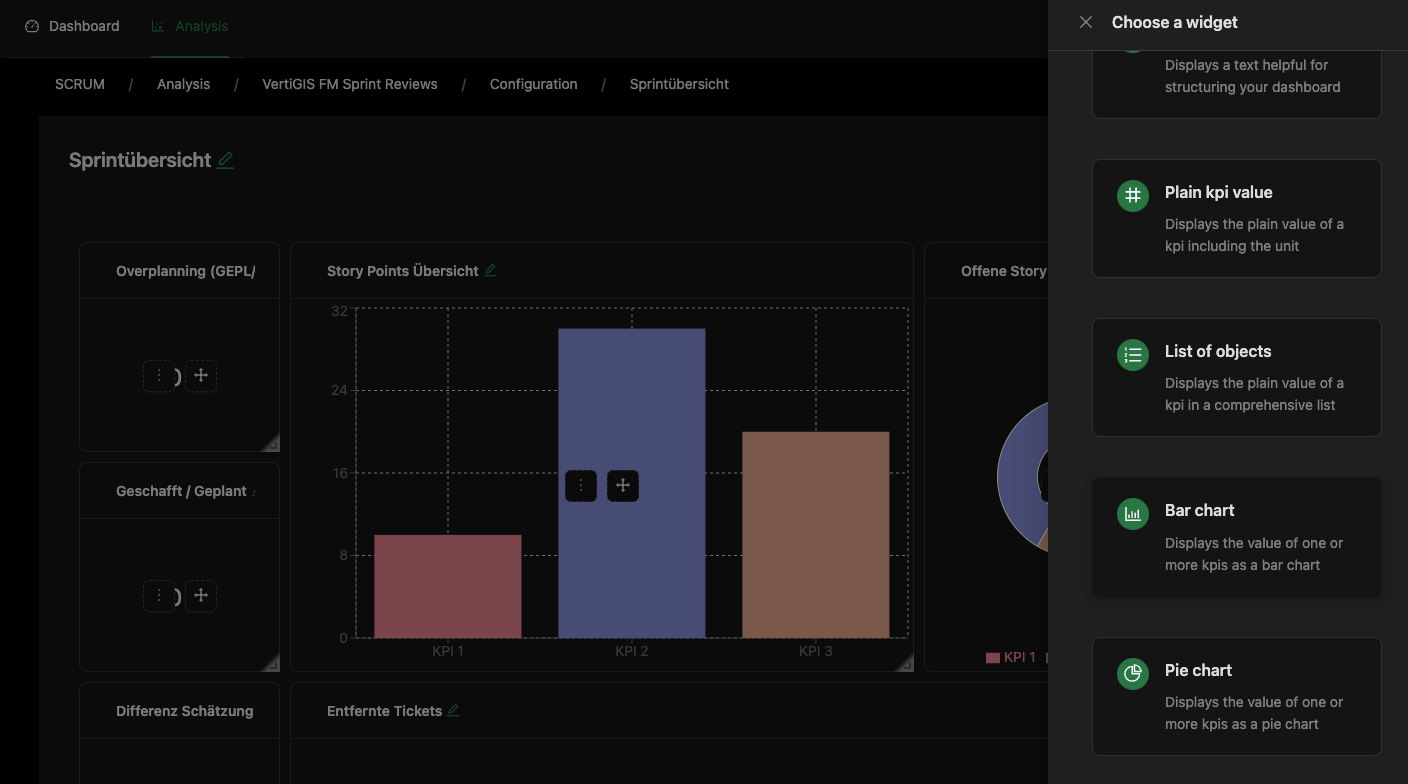
\includegraphics[width=0.6\linewidth]{Figures/DashboardsConfig.png}
    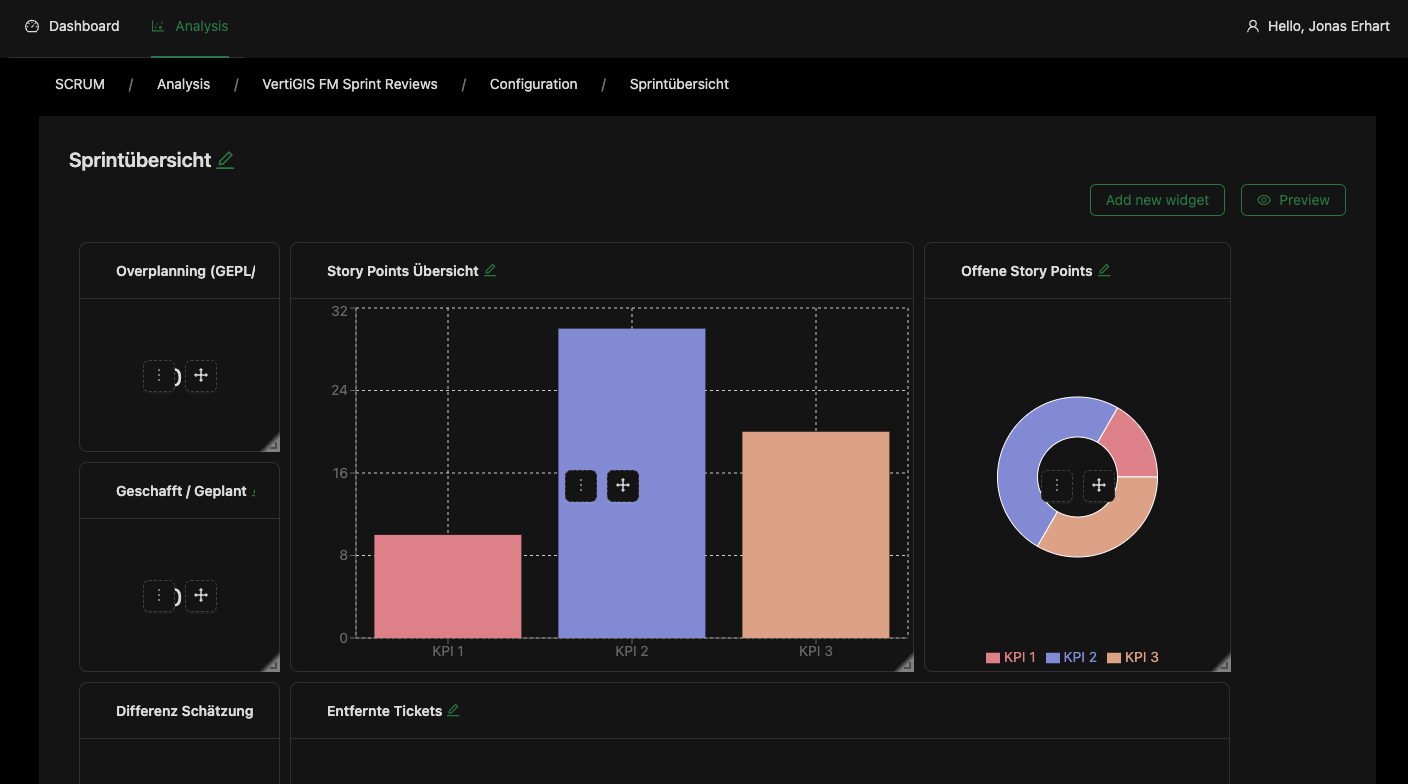
\includegraphics[width=0.6\linewidth]{Figures/DashboardConfigWidgets.png}
    \caption{Dashobard widget types and configuration}
    \label{fig:dashboards-config}
\end{figure}

\begin{figure}
    \centering
    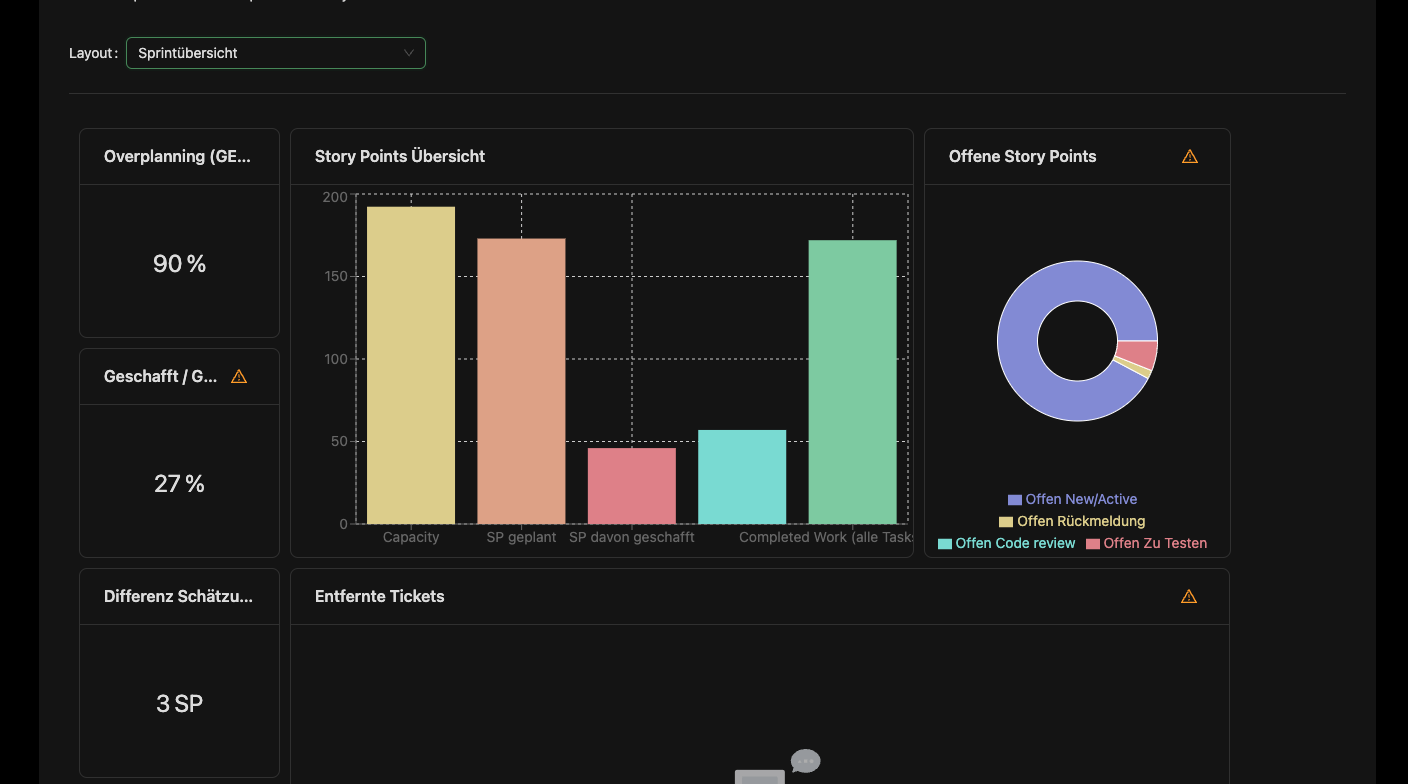
\includegraphics[width=1\linewidth]{Figures/DashboardApplication.png}
    \caption{Applied dashboard with real data}
    \label{fig:appl-dashboard}
\end{figure}
